
\par Las relaciones entre p\'aginas forman un grafo y resulta conveniente almacenarlos como una
matriz de uno y ceros, done el un uno en la poscici\'on $ij$ representa que la p\'agina $j$ apunta a la $i$.
A\'un as\'i esta implementaci\'ion tiene un problema: debe almacenar $n^2$ elementos, donde solo importan
$m$ (la cantidad de unos). En la pr\'actica, $m \ll n^2$ (ya que no todas las p\'aginas se relacionan
con todos). Es por esto que decidimos utilizar matrices \textit{ralas}: un tipo de matriz donde solo
importa donde hay unos, es decir, qu\'e p\'agina apunta a cu\'al.
\par Como primer acercamiento, evaluamos utilizar dos conocidos conocidos m\'etodos para el almacenamiento
de matrices ralas: CSR (Compressed Sparse Row) y CSC (Compressed Sparse Column). En el primer caso
nos encotramos con el problema de la dificultad de acceder a las colmunas, mientras que en el segundo,
las filas. consideramos de vital importancia poder acceder tanto a filas como columnas en un tiempo
razonable para operaciones tales como la multiplicación o la Eliminación Gaussiana.
\par Luego de evaluar los requerimientos, tanto de complejidad como de espacio utilizado, optamos
por implementar una estructura h\'ibrida entre un DOK (Dictionary Of Keys) y una lista de listas. 
Utilizamos una estructura que consiste en un diccionario de diccionarios: en el primero almacenamos
todas las filas y en el segundo sus elementos.
\par Respecto a la implementaci\'on, nos encontramos frente a la decisión de utilizar un diccionario ordenado
implementado sobre una estructura autobalanceada (\verb|std::map|) o un diccionario desordenado
implementado sobre una tabla de hash (\verb|std::unordered_map|). Si bien este \'ulitmo permite
el acceso en $O(1)$ en promedio frente al acceso en $O(\log n)$ del diccionario ordenado, 
no resulta f\'acil iterar eficientemete por lo que terminamos decidi\'endonos por la versi\'on autobalanceada.
\par Nuestro objetivo es resolver el sistema \ref{eq:Axx} o equivalentemente el sistema \ref{ipwd}, para lo cual 
resulta pr\'actico y eficiente utilizar Eliminación Gaussiana:

\begin{codebox}
\Procname{$\proc{Eliminación Gaussiana}(A)$}
\li \For $k \gets 1$ \To $n-1$
    \Do
\li     \For $i \gets k+1$ \To $n$
            \Do
\li         \For $j \gets k+1$ \To $n$
                \Do
\li                 $a_{ij} \gets a_{ij} - a_{ik}a_{kj}$
                \End
            \End
        \End
\end{codebox}

\par Como la matriz que utlizamos para almacenar la informci\'on es rala (no todos los elementos se encuentran definidos) por lo que 
adem\'as hay que asegurarse que los elementos est\'en definidos antes de operar con ellos. M\'as a\'un, dado que la resoluci\'on
del sistema no es m\'as que una aproximaci\'on, es necesario definir un $\varepsilon > 0$ para determinar qu\'e tan bien queremos que 
aproxime a la soluci\'on real; si bien un $\varepsilon$ m\'as chico producir\'ia una mejor aproximaci\'on, tambi\'en ralentiza la
ejecuci\'on del algoritmo. Es por esto, que junto con la esparsidad ($\delta = 1 - \frac{m}{n^2}$), decidimos hacer un an\'alisis
sobre el taman\~no del $\varepsilon$ por lo que el algoritmo de resoluci\'on queda:

\begin{codebox}\label{elimGaussRala}
\Procname{$\proc{Eliminación Gaussiana Rala}(A)$}
\li \For $k \gets 1$ \To $n-1$
    \Do
\li     \For $i \gets k+1$ \To $n$
            \Do
\li         \For $j \gets k+1$ \To $n$
                \Do
\li                \If $a_{ik}.definido()$ and $a_{kj}.definido()$
                        \Then
\li                        $mult \gets a_{ik}/a_{kk}$
\li                     \If $a_{ij}.definido()$
                            \Then
\li                          $a_{ij} \gets a_{ij} - mult*a_{kj}$
\li                     \Else
\li                          $a_{ij} \gets - mult*a_{kj}$
                \End
            \End
        \End
\end{codebox}
Observar que en ning\'un momento verificamos que $a_{kk}$ est\'e definido ya que la matriz permite hacer Eliminación Gaussiana sin necesidad
de pivoteo. (ver ap\'endice)
Luego para determinar las soluciones del sistema\cite{burden}:
\[
    x_n = \frac{a_{n,n-1}}{a_{nn}}
    \]
    \[
    x_i = \frac {a_{i,n+1} - \sum_{j=i+1}^{n} a_{ij}x} {a_{ii}}
    \]

Por \'ulitmo, normalizamos el vector $x$ de manera que $\sum^{n}_{i=1} |x_i| = 1$
\subsection*{Experimentaci\'on}

\par
En cuanto a la experimentaci\'on, pensamos en probar nuestra implementaci\'on de dos formas diferentes: de manera cualitativa y cuantitativa.
Para realizar el an\'alisis cuantitativo, generamos matrices aleatorias para luego variar los distintos parametros tales como probabilidad, 
tamaño de la matriz, cantidad de links y epsilon, para poder luego evaluar su incidencia. Para el an\'alisis cualitativo, construimos casos particulares
que nos resultaron interesantes analizar por diversos motivos.

\par 

Con respecto al an\'alisis cuantitativo, variamos los tres par\'ametros que considerados que podr\'ian ser interesantes de analizar:
el tama\~no de la matriz $n$, la cantidad de links $m$, la probabilidad $p$ y el $\varepsilon$.
\newline
En el primero de estos tests, creamos matrices de entrada aleatorias con tamaño $n$, probabilidad $p$ y $\varepsilon$ fijos, mientras variaban la cantidad de links $m$
de la matriz generada, es decir cambiando qu\'e tan rala es. A partir de esto, buscamos encontrar una relaci\'on entre la \textit{sparsity} y el tiempo.\newline
En este test nuestra expectativa fue encontrarnos con un incremento en el tiempo a medida 
que la \textit{sparsity} de nuestra matriz de entrada era menor, considerando que la
implementaci\'on fue diseñada para funcionar de manera eficiente en matrices de este tipo.

\par
Como segundo test, buscamos evaluar incidencia del par\'ametro $p$ en el tiempo de ejecuci\'on en una matriz de tamaño $m$, cantidad de links $n$ 
y $\varepsilon$ fijos.\newline
Al ver la ecuaci\'on \ref{ipwd} observamos que a medida que el par\'ametro $p$ decrece, tambi\'en lo hace el resultado de $pWD$ y, 
por la forma en que implementamos la igualdad, tener elementos m\'as pequeños en una matriz implica que m\'as elementos de la misma podr\'ian 
ser considerados ceros (dependiendo del $\varepsilon$ que estemos utilizando).\\
Esto nos hace pensar que resolver la ecuaci\'on anterior en con un $p$ relativamente pequeño  requerir\'ia menos tiempo.
Por \'ultimo, no quisimos pasar por alto otro aspecto que consideramos que consideramos que podr\'ia tener cierta relevancia en este test, el n\'umero de condici\'on. 
Como est\'a señalado en el ap\'endice, vimos que a menor $p$, mejor condicionada est\'a la matriz, entonces a medida que aumenta $p$, 
aumentar\'a tambi\'en la cota superior que tenemos para el n\'umero de condici\'on, con lo que nuestro calculo podr\'ia volverse menos estable, 
en el sentido de a pesar de no conocer el error, nos exponemos a que sea m\'as grande.
Si bien esto nos abre el camino a nuevas experimentaciones, entendemos que el eje de este trabajo no es este, es por esto que simplemente lo mencionamos como un posible tema de inter\'es para una pr\'oxima investigaci\'on.

\par
Como \'ultima prueba cuantitativa, mantuvimos fijos el tama\~no de la matriz $n$, la cantidad de links $m$, la probabilidad $p$ y variamos la precisi\'on del $\varepsilon$.
A la hora de realizar este test, estimamos que la variaci\'on del $\varepsilon$ no afectar\'a de manera significativa el tiempo de ejecuci\'on.

\par
Para analizar cualitativamente realizamos diversos tests a partir de casos de grafos particulares que nos resultaron importante destacar.
Elaboramos diferentes casos de test y tratamos de predecir el resultado del ranking para luego compararlo con los resultados obtenidos usando el algoritmo implementado. Para estos casos se decidió usar una cantidad chica de nodos debido a la dificultad para graficar y analizar grafos grandes.
Empezamos por casos muy simples como una cadena, sumando de a poco links para observar como influyen en el ranking.
Finalmente decidimos elaborar un grafo m\'as complejo con un esquema en el que se puede reconocer dos subgrafos principales m\'as densamente conectados internamente y con algunos pocos links entre ellos, incluyendo además nodos desconectados. La idea de estos últimos grafos fue simular, a pequeña escala, como funcionaría si tuviésemos por ejemplo dos sitios diferentes (por ejemplo uno de los subgrafos podría ser un portal de noticias), en los cuales hay muchas referencias a p\'aginas internas del sitio y espor\'adicamente links a p\'aginas de otros sitios. A su vez la p\'agina principal del portal puede ser referenciada desde otros sitios.
Otro test cualitativo que consideramos que pod\'ia aportarnos un panorama m\'as claro en cuanto al funcionamiento de nuestro rankeador, fue el caso de un grafo con donde el caminante podr\'ia seguir saltando entre p\'aginas relacionadas entre s\'i indefinidamente.
En el cuerpo principal del informe vamos a analizar casos tales como los de las figuras \ref{fig:Cadena simple}, \ref{fig:Cadena con nodo central}, \ref{fig:Nodos con muchos links salientes}, \ref{fig:Nodos con muchos links entrantes}. Para observar m\'as experimentos, dirigirse al ap\'endice.

\begin{figure}[H]
	\centering
	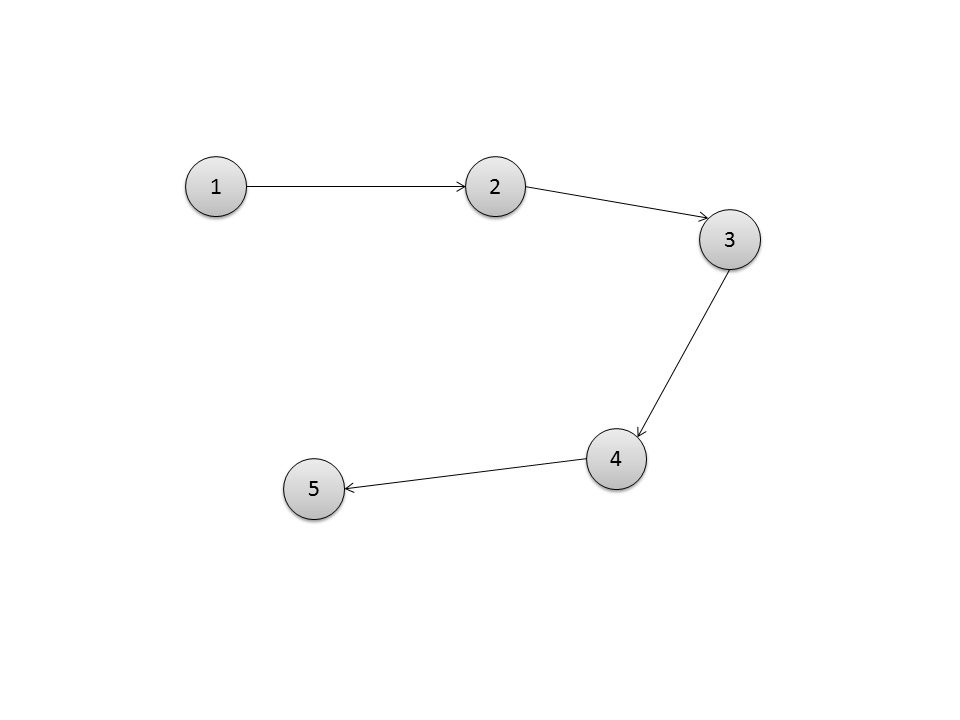
\includegraphics[width=0.7\textwidth]{img/cadena4.png}
	\caption{Nodos enlazados en una sola dirección}
	\label{fig:Cadena simple}
\end{figure}



\begin{figure}[H]
  \centering
    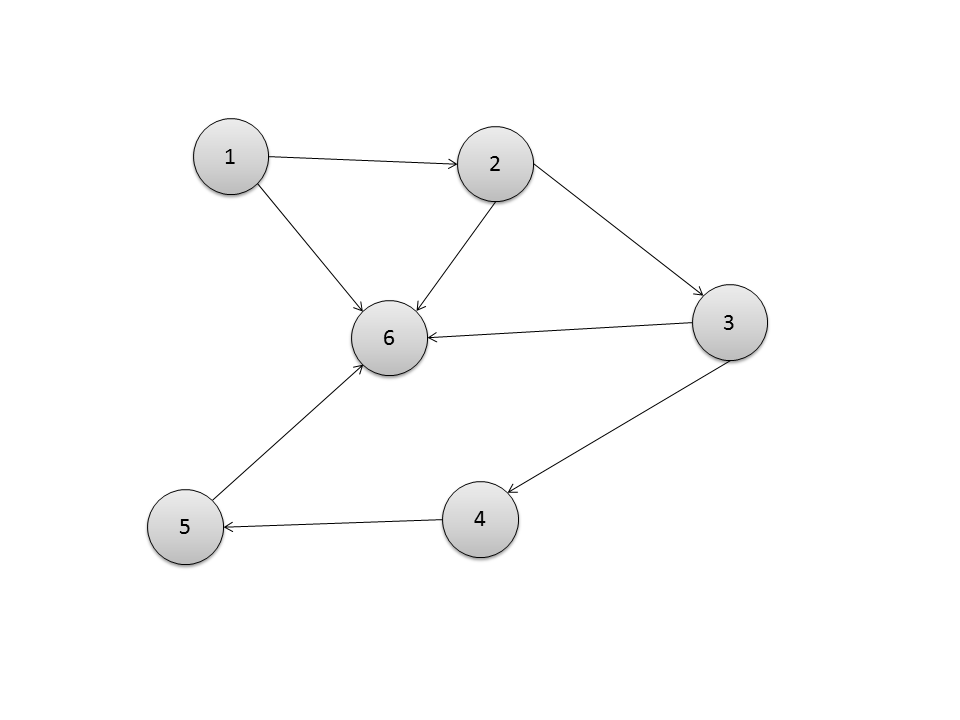
\includegraphics[width=0.7\textwidth]{img/Cadena6v2.png}
  \caption{Cadena con nodo central (caso 2)}
  \label{fig:Cadena con nodo central}
\end{figure}


\begin{figure}[H]
	\centering
	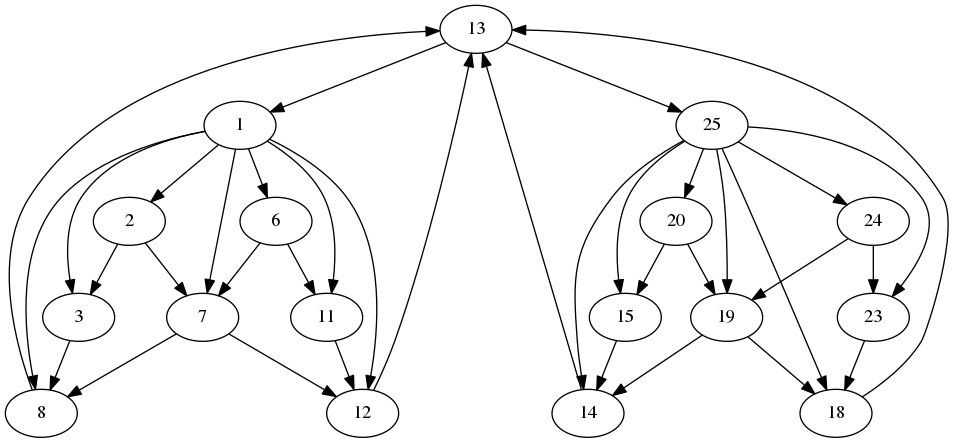
\includegraphics[width=0.9\textwidth]{img/links_salientes_25.png}
	\caption{Nodos con muchos links salientes}
	\label{fig:Nodos con muchos links salientes}
\end{figure}

\begin{figure}[H]
	\centering
	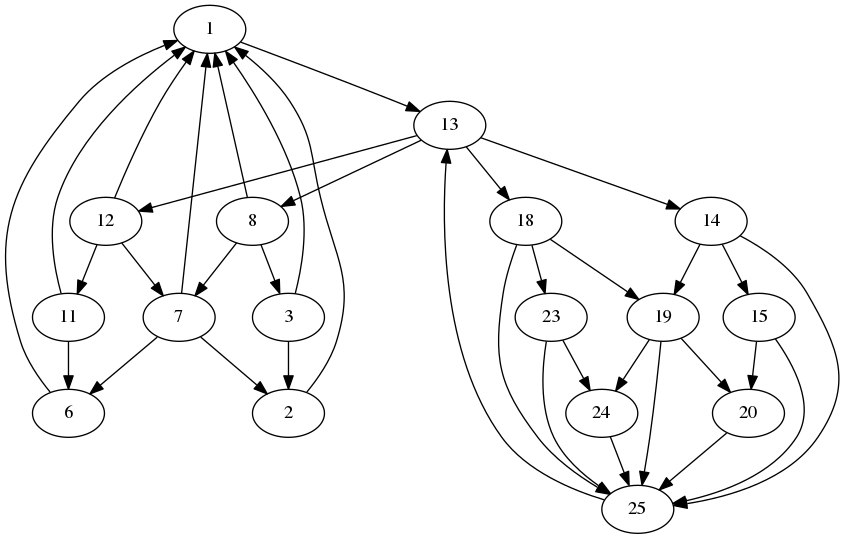
\includegraphics[width=0.7\textwidth]{img/links_entrantes_25.png}
	\caption{Nodos con muchos links entrantes}
	\label{fig:Nodos con muchos links entrantes}
\end{figure}
